\vskip0.5cm
\begin{columns}[t]
	\begin{Large}
	\begin{column}{0.025\textwidth}
	\end{column}
	\begin{column}{0.375\textwidth}
		Most popular approaches:
		\begin{itemize}
			\item[$\rhd$] \textit{Model augmentation}: improving prediction accuracy and control performance.
			\item[$\rhd$] \textit{Adaptive tuning} and \textit{parameter optimization}: parameters tuning (e.g. weights, costs, constraints).
			\item[$\rhd$] \textit{Safety}: learned-policy coupled with RHC controller, \textit{safety filter}.
		\end{itemize}

	\end{column}

	\begin{column}{0.6\textwidth}
		Our approach:
		\begin{figure}[h]
			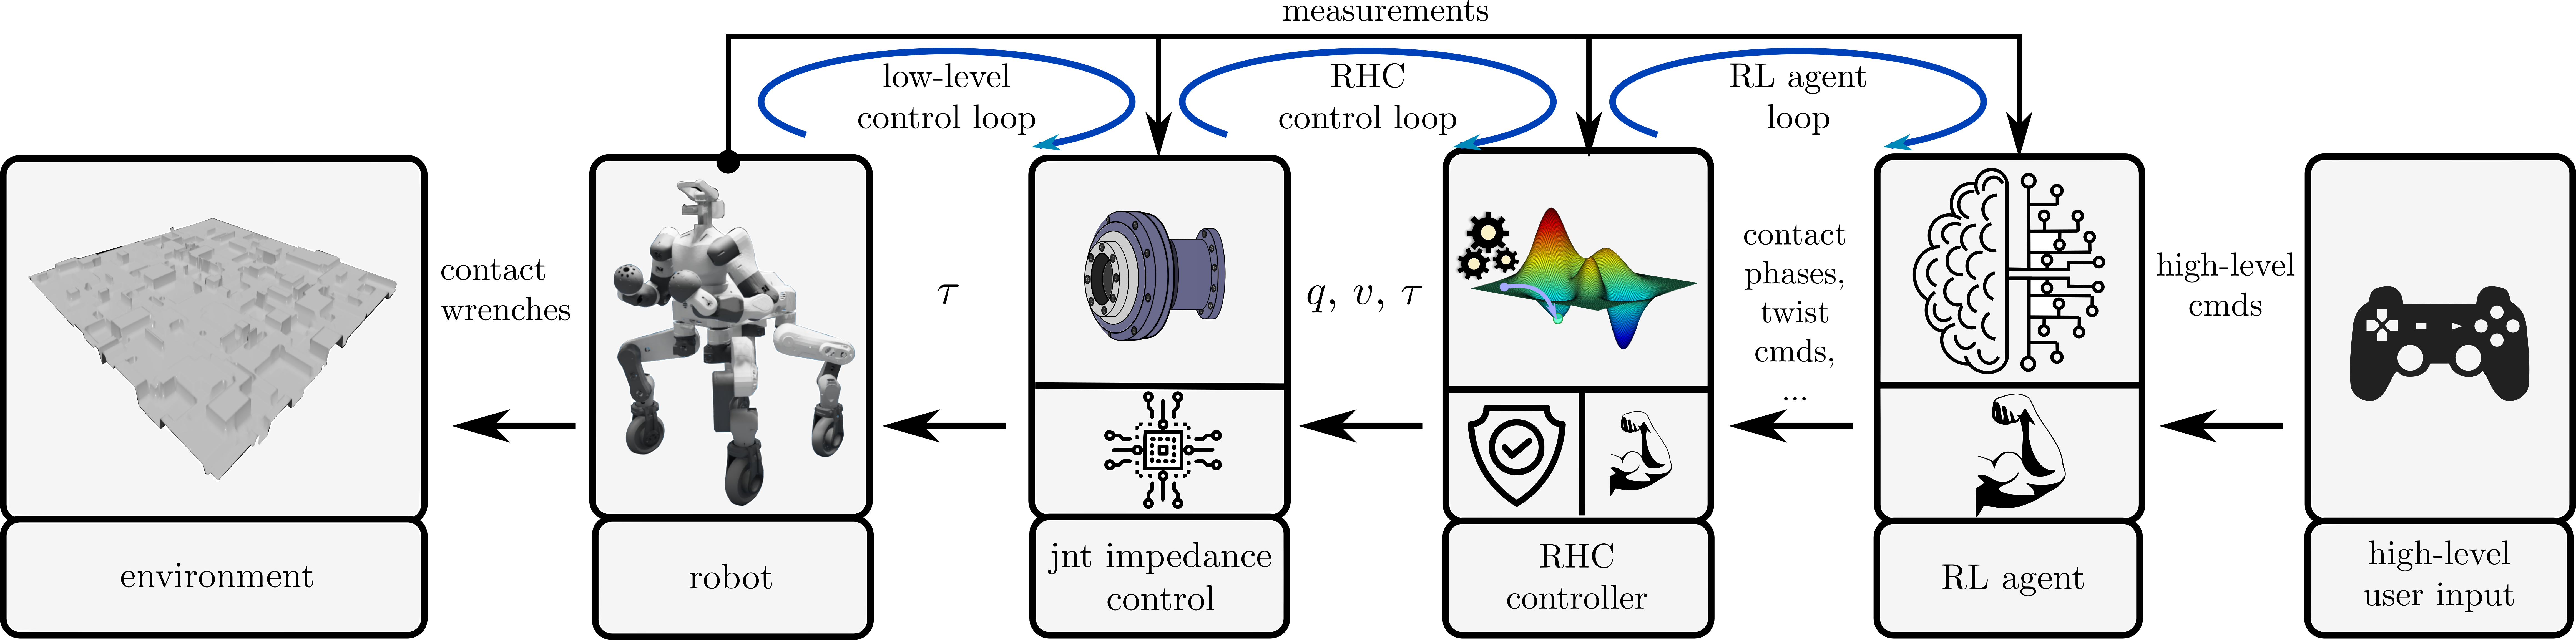
\includegraphics[width=0.8\textwidth]{docs/imgs/approach.png}
		\end{figure}
		\begin{itemize}
			\item[$\rhd$] \textit{Hierarchical coupling}: agent on top of RHC controller.
			\item[$\rhd$] RHC used as \textit{local} and \textit{safety-aware} controller.
			\item[$\rhd$] Agent for high-level task achievement and RHC \textit{performance} exploitation.
		\end{itemize}
		
	\end{column}
	\end{Large}
\end{columns}